%++++++++++++++++++++++++++++++++++++++++
\documentclass[letterpaper,12pt]{article}
\usepackage{showlabels}
\usepackage{natbib} %É uma ferramenta da bibliografia citep/ citet/ citeyear..
\usepackage[nottoc,notlof,notlot]{tocbibind} %Isto é para o índice, sem o tópico índicenoíndice
\usepackage{tabularx} %extra features for tabular environment
\usepackage{amsmath}  %improve math presentation
\usepackage{graphicx} %takes care of graphic including machinery
\usepackage[table]{xcolor} 
\usepackage[margin=1in,letterpaper]{geometry} %decreases margins
\usepackage{cite} % takes care of citations
\usepackage[final]{hyperref} % adds hyper links inside the generated pdf file
\usepackage{xspace}
\usepackage{subfig} % Serve para por 2 figuras lado a lado 
\usepackage{float}
\hypersetup{
	colorlinks=true,       % false: boxed links; true: colored links
	linkcolor=blue,        % color of internal links
	citecolor=blue,        % color of links to bibliography
	filecolor=magenta,     % color of file links
	urlcolor=blue         
}
%+++++++++++++++++++++++++++++++++++++++
\begin{document}
\title{\huge A Poluição do Meio Ambiente}
\author{R. Amorim nº 98197\\ G. Sousa 98321}
\date{\today}
\maketitle
\begin{figure}[h]
    \centering
    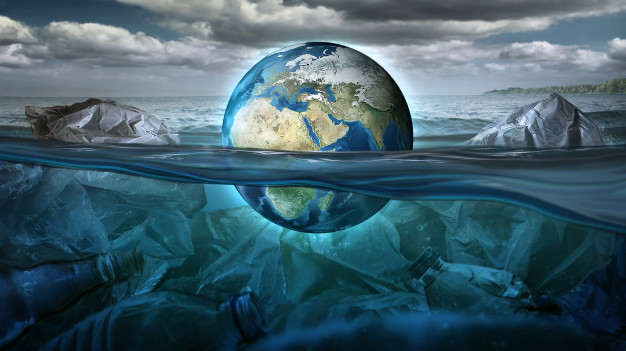
\includegraphics{PlanetaPlastico.jpg}
    \caption{\hbox{Planeta em Tempos de Crise}}
    \label{capa}
\end{figure}
%%%%%%%%%%%%Abtract%%%%%%%%%%%%%%%%%%%
\begin{abstract}
\centering
O seguinte trabalho irá abordar principalmente as invenções tecnológicas para a compensação de inúmeras \textbf{ações humanas inadequadas}, cujas deram origem a consequências \textbf{negativas}, estas serão referidas mais à frente com os \textbf{meios a adotar} para evitar mudanças drásticas.
\end{abstract}
%%%%%%%%%%%%%%%%%%%%%%%%%%%%%%%%%%%%%%%%
\newpage
%%%%%%%%%%%%%%%%%%%%%%ÍNDICE%%%%%%%%%%%%%%%%%%%%%%
\renewcommand{\contentsname}{Índice}
\tableofcontents

\listoffigures

\listoftables

%%%%%%%%%%%%%%%%%%%%FIM DO ÍNDICE%%%%%%%%%%%%%%%%%%%
\newpage
\section{Introdução}
\large O ambiente nem sempre foi um tema tão debatido como atualmente. Aliás até à revolução industrial este não era abordado, devido ao ambiente não ter impacto pela tecnologia usada nesses tempos. No entanto, com o passar dos anos e o desenvolvimento de mais e melhor tecnologia (em todas as áreas possíveis e imaginárias), a poluição e o uso de recursos considerados não reutilizáveis tem aumentado exponencialmente.
\par A exposição deste tópico é particularmente relevante, dado que, apesar da advertência de uma variedade enorme de cientistas que estudam áreas relacionadas com o ambiente, pouco ou até nada foi e está a ser feito para combater a degradação do ambiente.
\par É vital, portanto, criar este tipo de trabalhos para "abrir os olhos" de muita gente ou, por mais não seja, aumentar o conhecimento geral deste tópico, à semelhança de como já foi tentado de diversas formas, por exemplo, a criação de relógios \ref{fig:Relógio} que mostram que faltam 7 anos até ao "point of no return", ou seja, o ponto de rotura em que as alterações climáticas se tornam irreversíveis.
%%%%%%%%%%%%%%%%%%%%%%%%%%%%%%%%%%%%%%%%%%%%%
\section{Desenvolvimento}
\subsection{Meio Ambiente}
\citep{a2020_meio}
\large "Meio ambiente, do latim \textit{ambiens/ambientis}, que significa redor e envolver, refere-se ao conjunto de fatores físicos, biológicos e químicos que cercam os seres vivos, influenciando-os e sendo influenciados por eles. Pode ser entendido também como o conjunto de condições que permitem abrigar e reger a vida em todas as suas formas - os ecossistemas que existem na Terra."
Tal como foi referido nesta pequena descrição, o meio ambiente influencia os seres vivos que nele vivem e vice-versa. Isto implica que qualquer alteração realizada num dos lados, tem consequências diretas e indiretas no outro. Logo, ao acrescentar ao meio ambiente fatores prejudiciais como a poluição, vamos indubitavelmente ter consequências nocivas.
\par E, infelizmente, é isso que tem vindo a acontecer devido à influência da raça humana. Tendo como objetivo melhorar as nossas condições de vida, temos vindo a criar novos problemas de cerne ambiental.
%%%%%%%%%%%%%%%%%%%%%%%%%%%%%%%%%%%%%%%%
\subsection{Causas e Consequências}
{\large A maioria das {\bf causas}, senão a totalidade, surgiu a partir da mão humana, que geram resíduos, sejam eles materiais ou energéticos, estes para além de prejudicarem o meio ambiente também afetam a vida dos seres que nele residem. Como tal, para facilitar a compreensão dividimos em cinco grandes capítulos, onde interage com o sistema através de uma específica forma física e estes são:}
\vspace{0.3cm}
\begin{enumerate}
    \item Poluição aquática e terrestre
    \item Poluição do ar
    \item Poluição nuclear
    \item Poluição visual e sonora
\end{enumerate}
\paragraph 1. POLUIÇÃO AQUÁTICO E TERRESTRE
\par Optou-se por juntar estes 2 elementos da natureza, tendo em consideração que se relacionam diretamente, afetando um ao outro de forma mútua para o caso de se contaminar individualmente.
\par Portanto as principais causas são: herbicidas, pesticidas, derramamento de óleo, lixos industriais e domésticos, chumbo, mercúrio, zinco, detergentes, entre outros.
\vspace{1cm}
\begin{figure}[h]
    \centering
    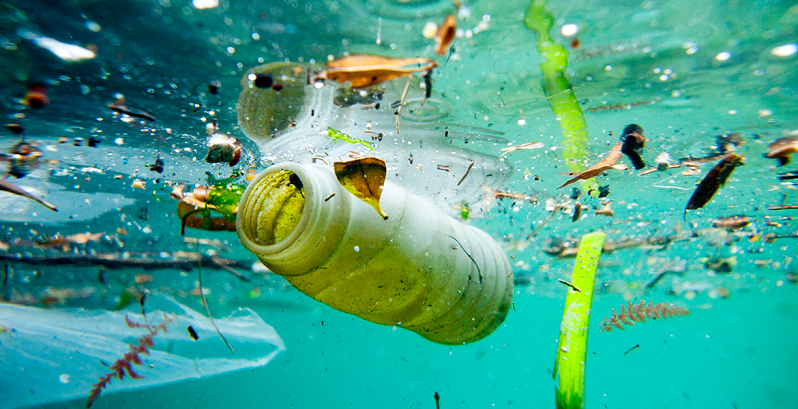
\includegraphics[width = 220px, height = 140px]{agua.png}
    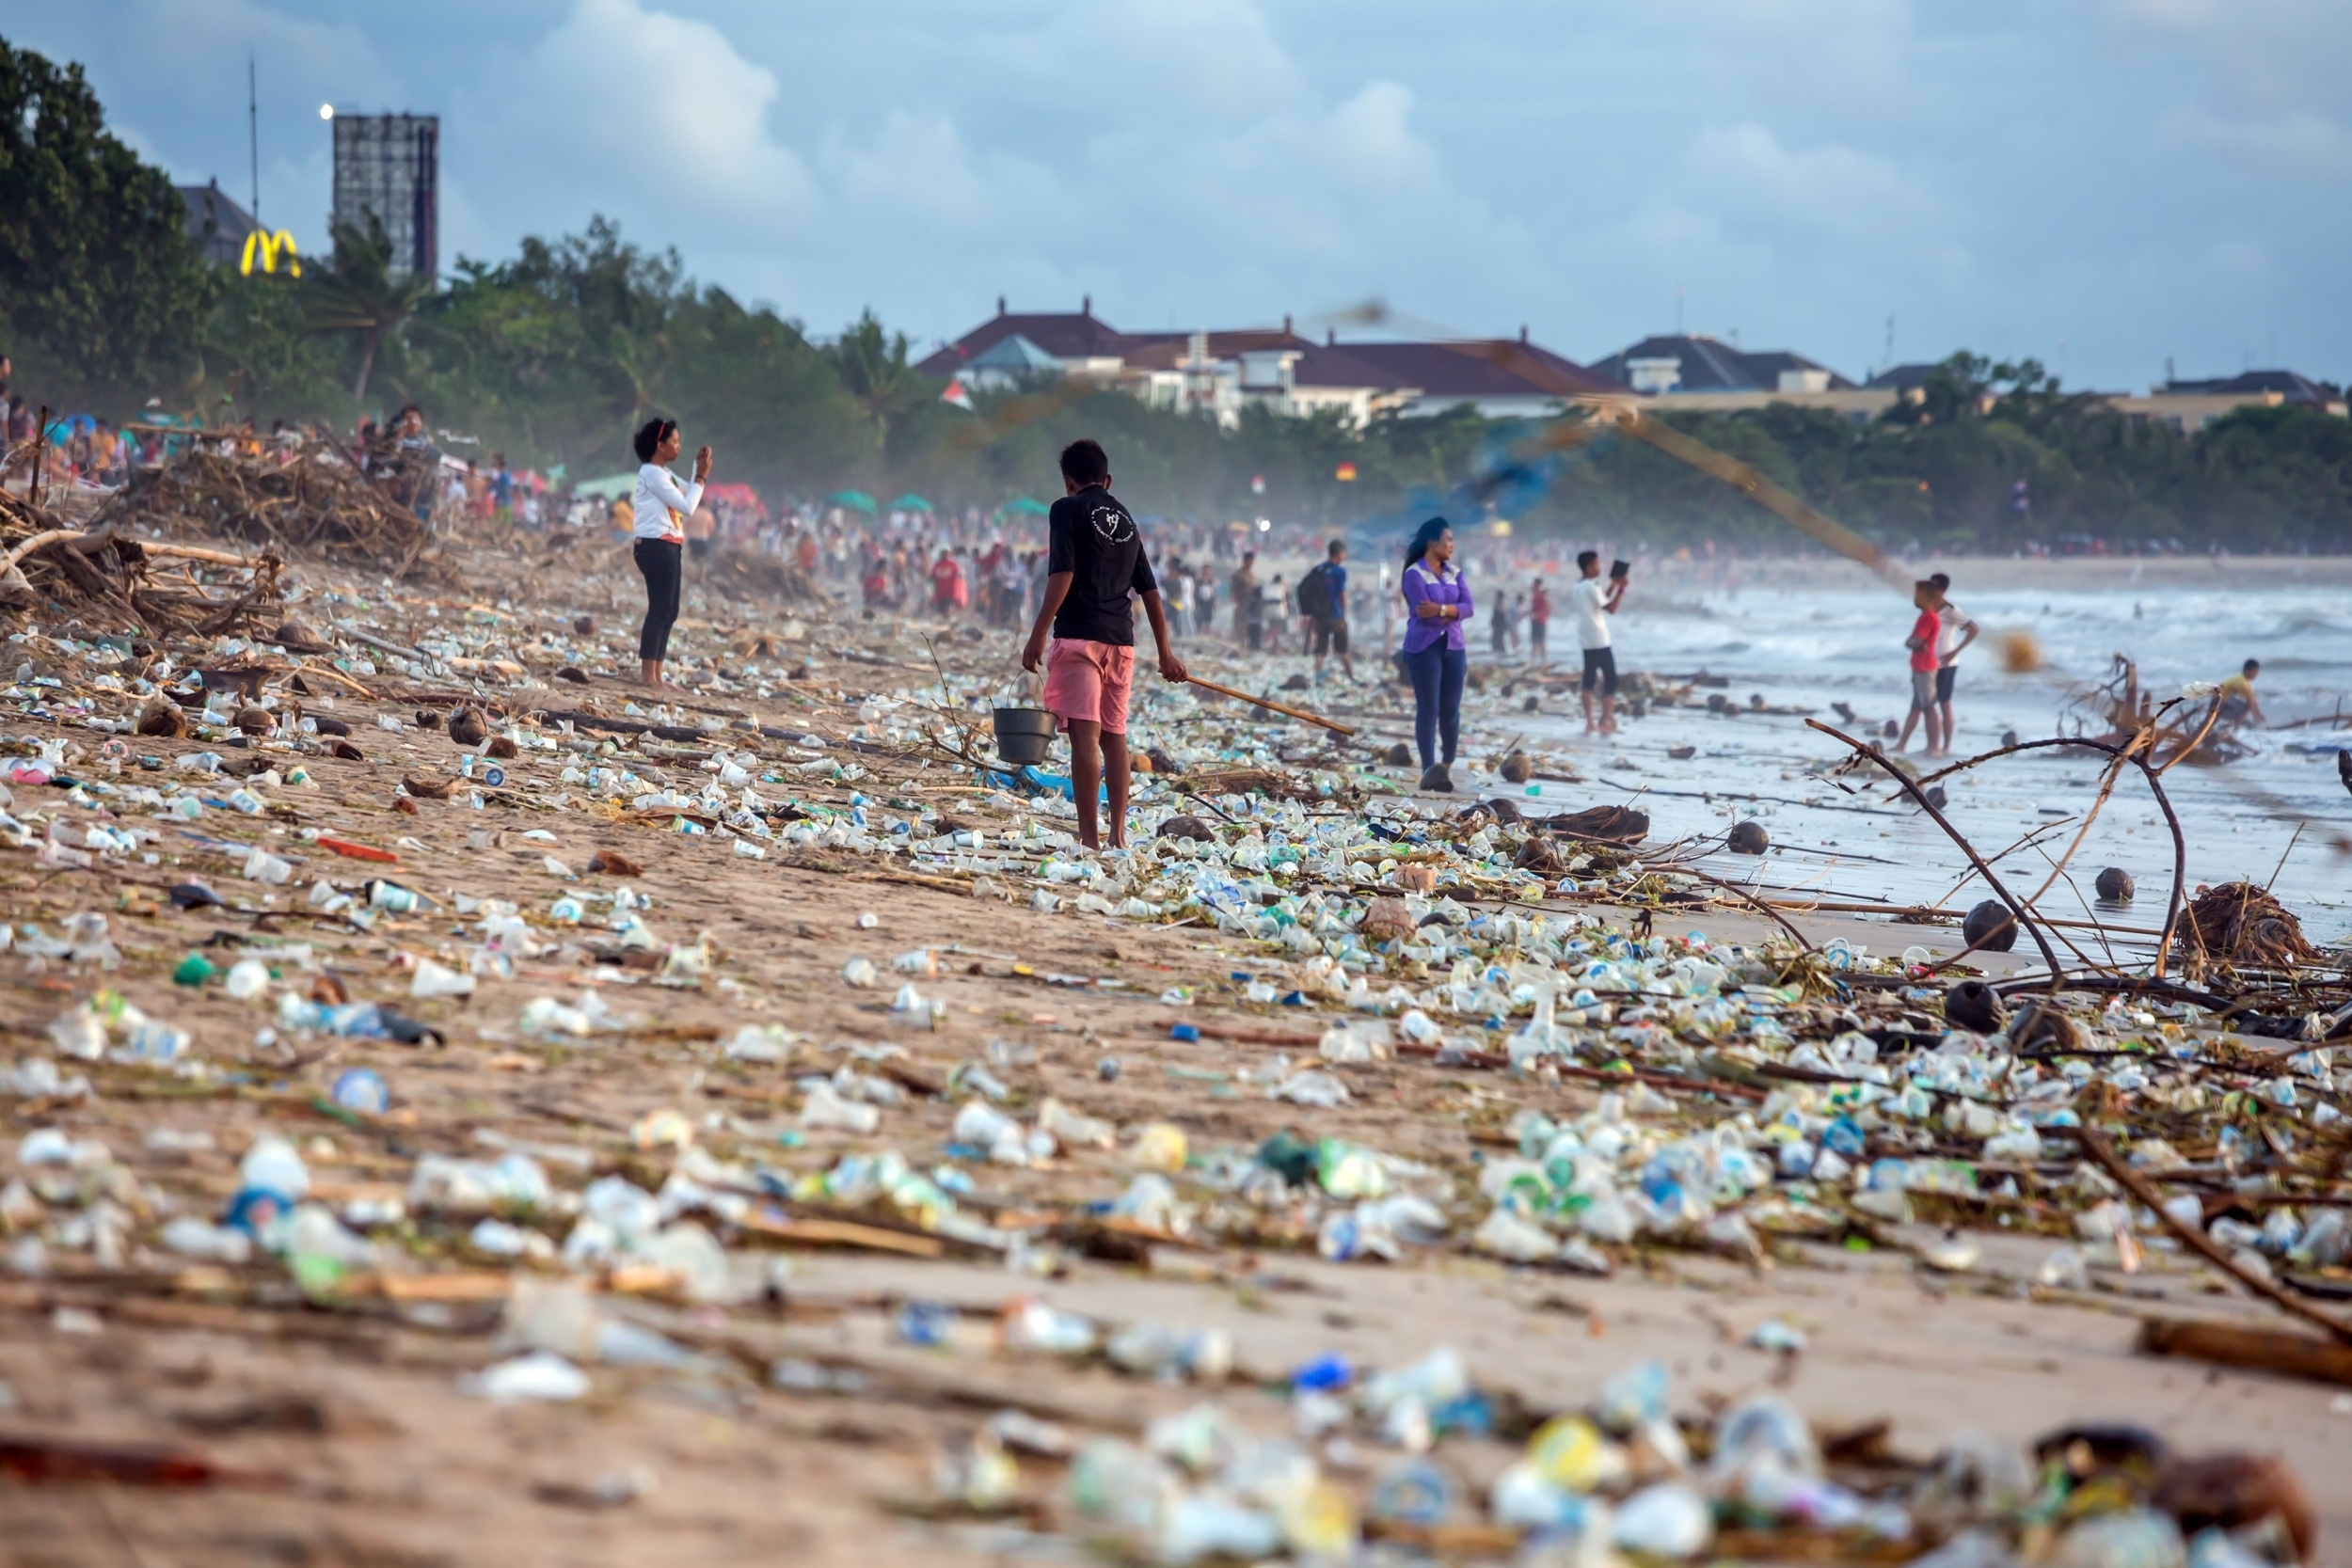
\includegraphics[width = 220px, height = 140px]{terramar.jpg}
    \caption{Lixo no Mar e na Terra}
    \label{fig:lixo na agua}
\end{figure}
%%%%%%%%%%%%%%%%%%%%%%%%%%%%%%%%%%%
%%%%%%%%%%%%%%%%%%%%%%%%%%%%%%%%%%%
\newpage
\paragraph 2. POLUIÇÃO DO AR
\par {\bf A queima de combustíveis fósseis} liberta CO2, que é um gás presente naturalmente na atmosfera que quando em excesso torna-se poluente. O gás carbónico junto com metano causa o efeito de estufa, que é essencial para a vida no planeta Terra, no entanto, a intensa atividade industrial e dos veículos conduz à produção destes gases em elevadas quantidades e a um efeito de estufa exacerbado, provocando, consequentemente, alterações climáticas, tais como, o \underline{Aquecimento Global}. \ref{fig:Radiação}
\par Por outro lado, as indústrias também emitem uma grande proporção de gases, tais como, nitrato e sulfato, que ao se combinarem com a atmosfera, originam \underline{Chuva Ácida}, causando a diminuição do pH do solo e da água, deste modo, temos respetivamente uma fraca fertilização e um aumento na mortalidade dos seres aquáticos.\\[0.3cm]
%%%%%%%%%%%%%%%%%%%%%%EmParalelo%%%%
\begin{minipage}{0.6\linewidth}
    \par \citep{rochavargasfogaa_clorofluorcarbonetos,cfcs}Existem outros fatores ao qual devem captar consideravelmente a nossa atenção temos, por exemplo, a \textbf{presença dos CFC's (CloroFluorCarbonetos)}  que são ligações químicas cujo em tempos devastou a camada de ozono induzindo o aumento da radiação ultravioleta, provocando o aumento das doenças cancerígenas da pele, cataratas, entre outros. Apesar da sua utilização ter sido diminuída, não apaga os danos denotados pelo buraco na camada de ozono sobre a Antártida de aproximadamente 29 milhões de quilómetros, atingindo o pico em 2000 que se foi propagando durante 50 anos.\\[0.3cm]
\end{minipage}
\begin{minipage}{0.44\linewidth}
    \begin{figure}[H]
        \centering
        
\includegraphics[scale = 0.2, angle = 90]{cfc.jpg}
        \caption{Efeito do CFC}
        \label{fig:CFC}
    \end{figure}
\end{minipage}
%%%%%%%%%%%%%%%%%%%EmParalelo%%%
\par Para remediar o resultados anteriores, executaram novas fórmulas genéricas (HCFC) para substituir a sua utilidade (Sprays e/ ou gases de refrigeração) reduzindo assim em 10\% no impacto causado pelo CFC.
\par Estatisticamente, de acordo com a Organização Mundial da Saúde (OMS), a poluição do ar é responsável por mais de sete milhões de mortes por ano no mundo, superando a Malária e a ADIS. Para que não basta, existem também estudos que revelam que este tipo de poluente chegam a atingir todos os órgãos do corpo humano.

%%%%%%%%%%%%%%%%%%%%%%%%%%%%%%%%%%%%%%%
%%%%%%%%%%%%%%%%%%%%%%%%%%%%%%%%%%%%%%%
\newpage
\paragraph 3. POLUIÇÃO NUCLEAR
\par Ou também conhecida como \textbf{Poluição Radioativa} foi descoberta no ano 1896 e desde então foram desenvolvidas tecnologias para o domínio da radioatividade e da energia gerada na transformação de átomos.
Essa tecnologia trouxe vários benefícios tais como: Radioterapia; Radiografia; Geração de Energia; Esterilização de materiais; Conservação de alimentos; Uso militar (Bombas); Entre outras.
\par Pelo seu alto grau de periculosidade, é considerado o pior tipo de poluição. Como todos sabem a radiação ocorre inevitavelmente, sendo algo sem alarmar, contudo as atividades humanas emitem em altas concentrações. Daí geram um lixo, que deve ser descartado num local apropriado e isolado, para não haver perigo de contacto com tal. Estas usinas nucleares geram 17\% da energia elétrica do mundo.
\begin{figure}[h!]
    \centering
    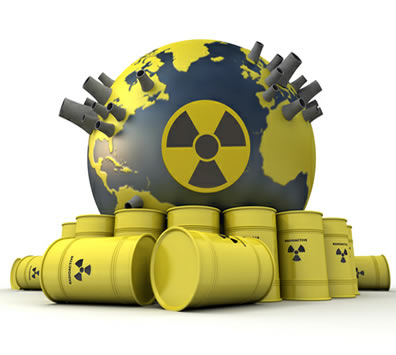
\includegraphics[scale = 0.35]{pnuclear.jpg}
    \caption{Poluição nuclear}
    \label{fig:7}
\end{figure}
\paragraph 4. POLUIÇÃO VISUAL E SONORA
\par Decidimos agrupar estes 2 tipos de poluição tendo em conta a sua extrema ligação. Surgem devido ao excesso de cartazes de publicidade, edifícios iluminados e luzes durante a época noturna, sem mencionar o rebuliço causado pelo trânsito automobilístico, na altura que a maioria dos animais descansam.
\par  Nós somos fotossensíveis, ou seja, sensíveis à luz e portanto devemos repousar num ambiente escuro. O mesmo acontece no que diz ao som. De maneira semelhante ocorre com a maioria dos animais. Estes devido ao excesso de luz e som, perdem a noção de quando devem descansar e ficam desorientados e em vários casos são incapazes de dormir o que os deixa debilitados.
%%%%%%%%%%%%%%%%%%%%%%%%%%%%%%%%%%%%%%%%%%%%%
%%%%%%%%%%%%%%%%%%%%%%%%%%%%%%%%%%%%%%%%%%%%%
\newpage
\subsection{Inovações tecnológicas}
\par Sugere-se a visualização de um vídeo que abrange tudo o que irá ser abordado posteriormente.
\begin{center}\fbox{\href{https://www.youtube.com/watch?v=PGS1ksdxS68&t=2s&ab_channel=BoredBadger}{Clique Aqui}}
\end{center}
\vspace{0.2cm}
\par \citep{badger_2019_will} O vídeo mostra outras ideias para além das referidas neste documento, tais como, a {\bf Polinização das abelhas}; Caneta que possui uma {\bf tinta sustentável}, produzida através da poluição que um carro faz numa hora, etc.

%%%%%%%%%%%%%%%%%%%%%%%%%%%%%%%%%%%%%%%%%%%%%%%%
\subsubsection{Relógio do Clima}
\par \citep{dures_2020_um}Este não é um relógio vulgar, tendo em consideração que não mostra as horas, mas sim uma contagem regressiva, que por sua vez indica aproximadamente um parcial de 7 anos até ao momento, mas pode estabilizar garantindo uma maior durabilidade à nossa existência e do próprio planeta, mas para tal temos que advertir toda a população que se cada um fizer a sua parte, isto é, se trabalharmos em {\bf equipa} com a devida responsabilidade e consciência, garantimos efetivamente uma esperança imprescindível. 
\begin{figure}[!htb]
    \centering
    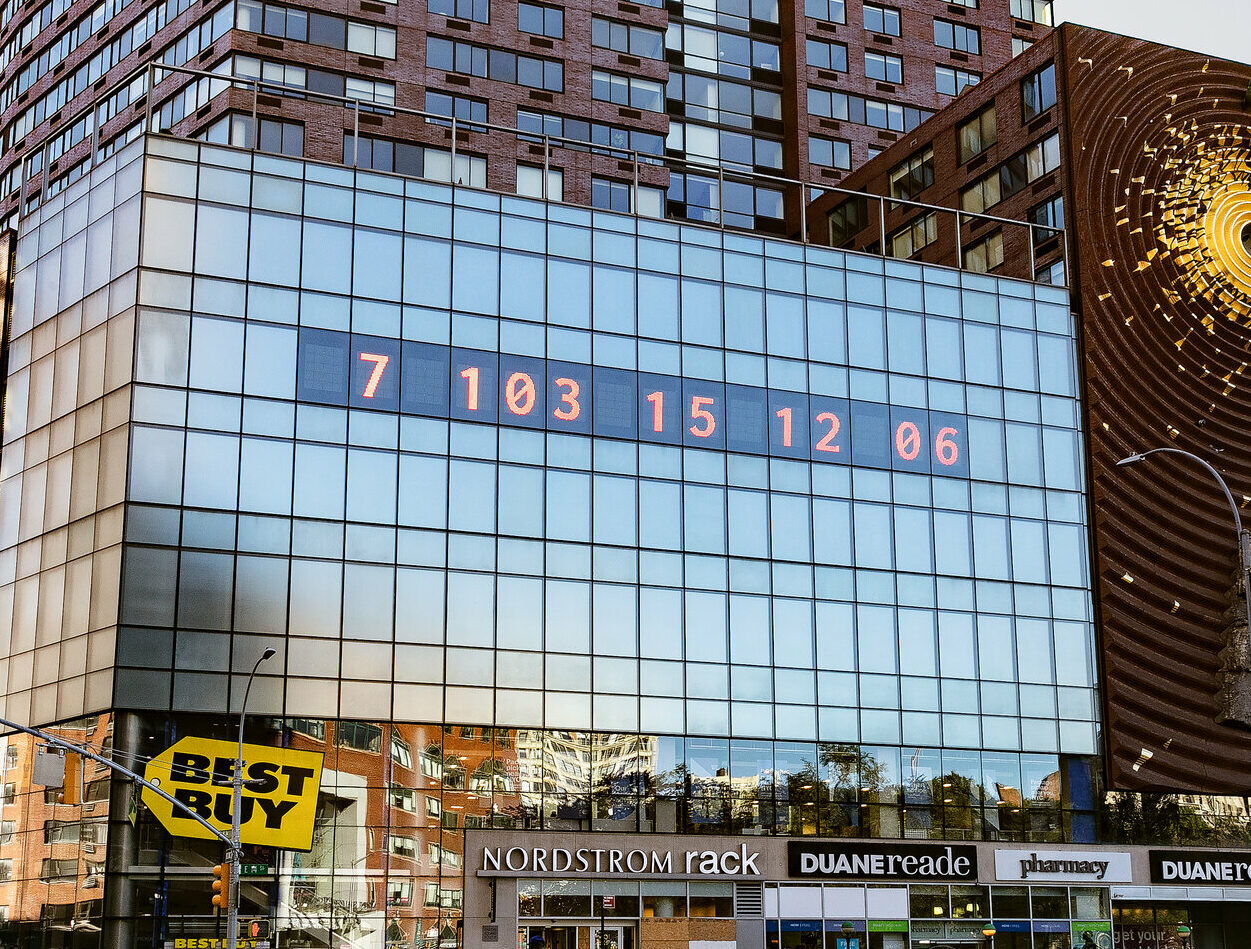
\includegraphics[scale = 3]{Relogio.jpg}
    \caption{Relógio da catástrofe climática}
    \label{fig:Relógio}
\end{figure}

%%%%%%%%%%%%%%%%%%%%%%%%%%%%%%%%%%%%%%%%%%%%%%
%%%%%%%%%%%%%%%%%%%%%%%%%%%%%%%%%%%%%%%%%%%%%%
\newpage
\par\large{\textbf{No fundo qual é a função deste relógio?}}
\par O relógio é uma das diversas plataformas que se conseguiu criar, este serve como um \underline{lembrete visual} de grande dimensão ao que se tenciona adotar por diversas cidades em todo o mundo para que assim alcance mais olhos, elucidando todos daquilo que realmente atravessamos, ou seja, é um {\bf estado crítico}, que de certa forma, revela literalmente uma corrida contra o tempo. 
\par Caso cheguemos ao "Point of no return" devido à excessiva emissão de carbono o previsto de acontecer é um aumento de 1,5 graus Celsius, por outras palavras, surge uma instabilidade climática ao ponto da existência terrestre se tornar \underline{HISTÓRIA}.\\[0.3cm]
\par {\bf Como funciona a destruição da camada de ozono?}
\par As maiores fontes de agravamento são os gases poluentes, por exemplo, como já referido os CFC \ref{fig:CFC}, ou seja, esses gases acabam por destruir a camada de ozono que, consequentemente, permite cada vez mais a entrada de radiação \ref{fig:Radiação} causando o efeito de estufa, o que nos leva aos {\bf cálculos do  climate clock}.
\begin{figure}[htp]
    \centering
    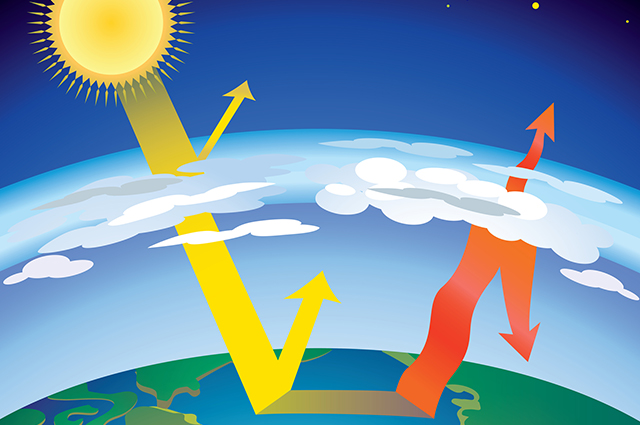
\includegraphics[width = 400px, height = 170px]{eq2.jpg}
    \caption{Radiaçao absorvida pela terra}
    \label{fig:Radiação}
\end{figure}
\par Por fim o relógio não nos garante o bem estar na presença do tempo registado no painel do edifício, mas sim, antes que seja tarde demais, {\bf definir medidas drásticas}, para isso existem voluntariados, sites de iniciativas, campanhas de apoio e ideias para contribuir, instruções online para aderir ao relógio ilustrado em casa, entre outros.
%%%%%%%%%%%%%%%%%%%%%%%%%%%%%%%%%%%%%%%%%%%
%%%%%%%%%%%%%%%%%%%%%%%%%%%%%%%%%%%%%%%%%%%
\newpage
\subsubsection{Enzima que consome plástico}
\par \citep{wellewwwdwcom_2018_cientistas} Investigadores britânicos e norte-americanos conseguiram criar uma enzima com capacidade de metabolizar o plástico. Esta descoberta, que ocorreu acidentalmente, garantiu um grande avanço pois, enquanto, que antes o plástico demorava 400 anos a se decompor, agora demora apenas poucos dias.\\[0.1cm]
%%%%%%%%%%%%%%%%%%%%%%ImgEmParaleloComOTexto%%%
\begin{minipage}{0.5\linewidth}
\vspace{0.3cm}
    \par A versão original foi encontrada, num centro de reciclagem japonês, pelos investigadores da Universidade de Portsmouth e do Laboratório Nacional de Energia Renovável dos EUA, adicionaram à enzima alguns aminoácidos que estimulou de forma mais acelerada e eficiente, utilizando um raio-X de brilho dez bilhões de vezes mais forte que o do Sol, assim conseguiram elaborar um modelo tridimensional de alta resolução da dita “Super Enzima” conhecida como \textit{Ideonella Sakaiensis}, decifraram a estrutura detalhada dessa substância orgânica. Com o acrescento de a terem mesmo potenciado.\\[0.1cm]
\end{minipage}
\begin{minipage}{0.55\linewidth}
\begin{figure}[H]
    \centering
    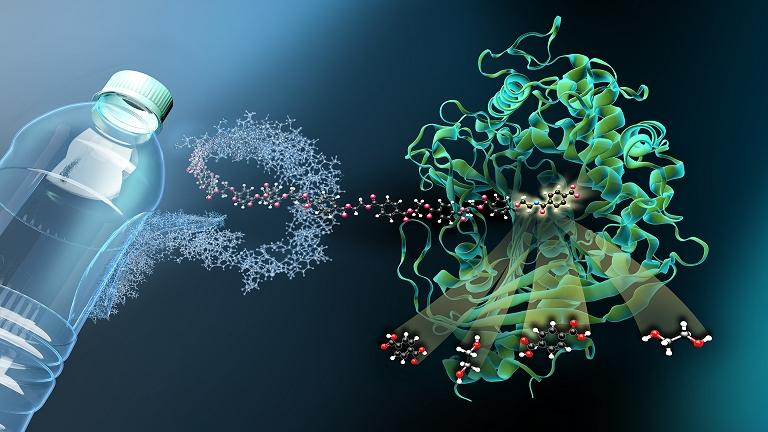
\includegraphics[width = 220px, height = 230px]{enzima.jpg}
    \caption{Ideonella Sakaiensis}
    \label{fig:enzima}
\end{figure}
\end{minipage}
%%%%%%%%%%%%%%%%%%%%%%%%%%%%%%%%EmParalelo%%%
\par Em 2017, os investigadores da Universidade de Aveiro descobriram no fundo dos oceanos um fungo que degrada plástico, portanto garantiram mais um meio prometedor de combater a propagação do plástico.
\par Essa equipa da UA simulou num laboratório uma situação idêntica à do oceano com plástico. Comprovou que, após vários testes, havia uma relação inversamente proporcional entre a quantidade de plástico e a de fungos.
\par O objetivo será melhorar esta enzima para que possa ser usada à escala industrial permitindo a {\bf reutilização do plástico} que neste momento demora centenas de anos a degradar-se.
\par Segundo a estatística das organizações ambientais são fabricadas {\bf 300 milhões de toneladas de plástico, por ano, em todo o mundo, sendo que destas cerca de 8 milhões terminam nos oceanos}.
%%%%%%%%%%%%%%%%%%%%%%%%%%%%%%%%%%%%%%%%%%%%%
%%%%%%%%%%%%%%%%%%%%%%%%%%%%%%%%%%%%%%%%%%%%%
\newpage
\subsubsection{Sistema de Ocean CleanUp}
\par \citep{n_2019_mquina}Este sistema chama-se "001/B" criado pela fundação cujo nome é "Ocean CleanUp", faz aquilo que está referido no nome da fundação limpa os oceanos. Mas surge agora a questão, {\bf como é que efetivamente faz essa limpeza?}
\par Bem, a ideia original foi proveniente de um adolescente holandês em 2012, Boyan Slat, tendo a primeira apresentação do sistema acontecido numa TedTalk. Aí o criador da ideia explica a forma como se utilizariam as próprias correntes marítimas para capturar o lixo indesejado numa barreira que se estende em 600 metros de comprimento e 3 metros de profundidade, \underline{em forma de U}.
\begin{figure}[h]
    \centering
    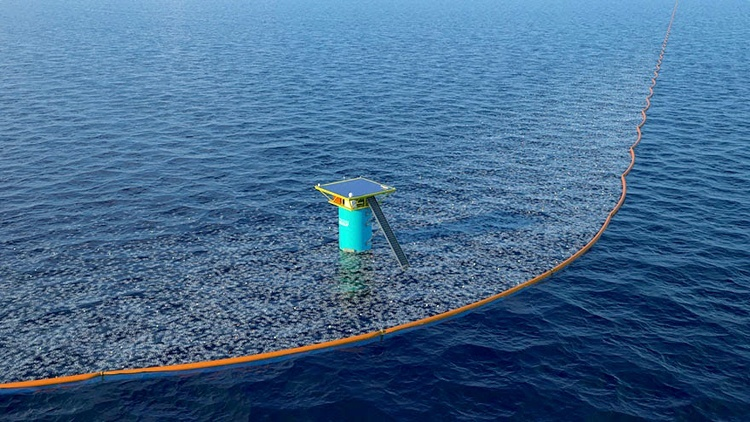
\includegraphics[width = 190px, height = 120px]{OCup1.jpg}
    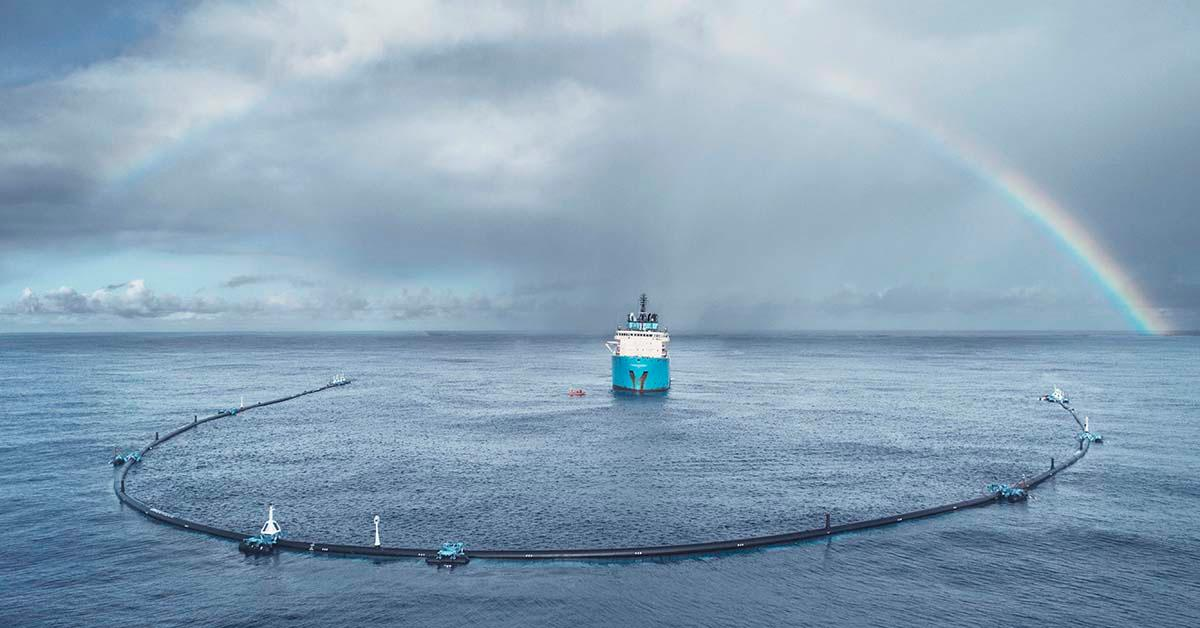
\includegraphics[width = 210px, height = 120px]{OCUp.jpg}
    \caption{Sistema do Ocean CleanUp em forma de U}
    \label{fig:OC}
\end{figure}
\par Funciona como uma rede e apanha entre os mais diversos resíduos, também os microplásticos muito nocivos a ingestão por seres vivos. Após alguns anos de testes, obtevê-se a versão que está atualmente em utilização e funcional, tendo sido utilizada na maior acumulação de plásticos do mundo que tem 17 vezes o tamanho de Portugal continental, a Madeira e os Açores juntos.
\par Este sistema tem definido múltiplos benefícios onde os principais são, funcionamento {\bf autónomo} o que retira uma grande parte da mão de obra associada a um projeto desta escala. De seguida, a situação da poluição marítima tem vindo a agravar seriamente, logo é fulcral a sua utilização, pois facilita o trabalho de {\bf recolher lixo}, onde simplesmente andava à deriva sem o menor tipo de controlo.

%%%%%%%%%%%%%%%%%%%%%%%%%%%%%%%%%%%%%%%%%%%%%
%%%%%%%%%%%%%%%%%%%%%%%%%%%%%%%%%%%%%%%%%%%%%
\newpage
\subsubsection{Roupas Energéticas}
\par \citep{rosa_2012_cientistas, sousa_2019_camiseta,ciclovivo_2017_cientista}
Dois estudos científicos certificaram avanços no que diz respeito à redução de poluição, criando roupa, mais especificamente, novos tecidos com propriedades de armazenar e/ou criar energia, obtendo-a a partir da radiação solar e corporal.
\par O conceito por detrás do seu funcionamento é a diferença entre a temperatura ambiente e corporal, em especial, enquanto se pratica qualquer tipo de {\bf atividade física}, tem-se que o calor corporal aumenta e, desse modo, gera energia que é redirecionada para o tecido. Contudo, esta tecnologia tem desvantagens em termos da quantidade, pois é menor que outros materiais criados com o mesmo propósito, outro ponto a destacar é a dificuldade das lavagens. Confirma-se que, após a análise deste projeto, estamos ainda numa fase inicial onde tudo são só ideias.
\begin{figure}[h!]
    \centering
    \includegraphics[width = 200px, height = 150px]{Roupa Energética.jpg}
    \caption{Exemplo de Roupa Energética (A partir da Energia Solar)}
    \label{fig:Roupa Energética}
\end{figure}
\par Em 2012, um grupo de cientistas criou uma camisola com o intuito de armazenar energia, para isso transformaram as fibras de algodão num {\bf supercapacitor} de alto desempenho. Apontam que, o processo é simples e de baixo impacto ambiental, pois não requer grande quantidade de energia, não depende de substâncias químicas nocivas e não produz resíduos perigosos, o que é claramente vantajoso ao ambiente. No entanto, não tem capacidades de gerar energia ao contrário da camisola relativa ao próximo tópico.
\par Segundo um artigo de 2017, criaram um tecido que utiliza filamentos de cobre extremamente finos, em fitas que possuem uma {\bf célula solar} e {\bf camadas de armazenamento}, para gerar e armazenar energia. Adicionalmente, este tecido pode ser utilizado da maneira tradicional sem qualquer perda de eficácia a nível de armazenamento e produção de energia.
%%%%%%%%%%%%%%%%%%%%%%%%%%%%%%%%%%%%%%%%%%%%
%%%%%%%%%%%%%%%%%%%%%%%%%%%%%%%%%%%%%%%%%%%%
\newpage
\subsubsection{Comboios de Energia Eólica}
\par \citep{rosa_2017_trens,camargo_2015_trens}Por toda a Europa, as velhas locomotivas com {\bf motor diesel} desapareceram praticamente para dar lugar {\bf às elétricas}, o que ajudou a estabelecer o \underline{EQUILÍBRIO}, no entanto, os caminhos ferroviários não deixam de ser responsáveis indiretamente, pois emitem poluentes resultantes da circulação, estima-se que por ano um comboio expõe cerca de {\bf 1,2 bilhões de kWh de energia elétrica}, gerada por fontes eólicas são transportados anualmente pela NS, a maior empresa ferroviária holandesa.
\par A Holanda é uma exceção ao referido atrás, tendo sido delineado um objetivo de reduzir o desperdício e simultâneamente gerar "energia limpa", no fundo passou a não emitir nada, isto é, foi palco de um projeto onde 100\% das energias são renováveis, ou seja, utilizando energia ‘verde’ fornecida pela empresa Eneco, desta forma pretende-se alcançar a neutralidade de carbono.
\begin{figure}[!htb] 
    \centering
    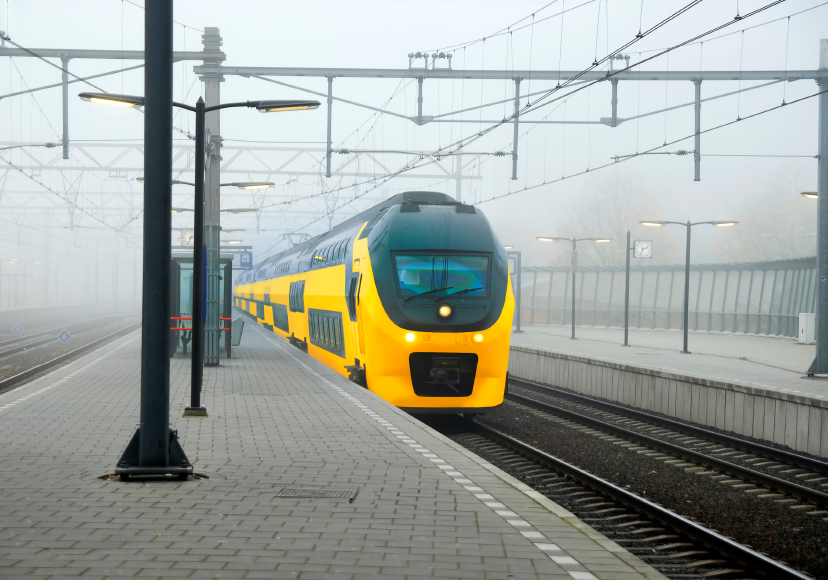
\includegraphics[width = 150px, height = 150px, angle = 20]{comboio.jpg}
    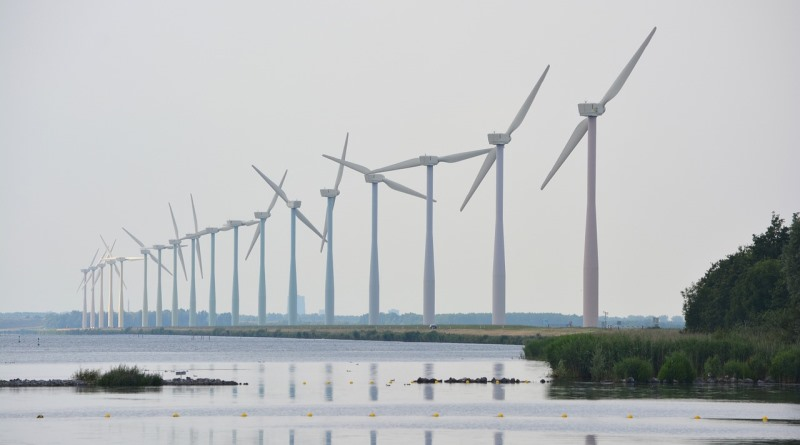
\includegraphics[width = 200px, height = 150px, angle = 340]{eolicas.jpg}
    \caption{Comboios movidos com energia eólica}
    \label{Energia renovável}
\end{figure}
\par Acredita-se que o sucesso deste projeto {\bf inspire} outras cidades, por exemplo, na Alemanha prevê-se igual meta para 2050. Pode-se considerar que nos encontramos perante um grande passo sem contribuir para as alterações climáticas \ref{fig:Radiação}.
%%%%%%%%%%%%%%%%%%%%%%%%%%%%%%%%%%%%%%%%%%%%%%%
%%%%%%%%%%%%%%%%%%%%%%%%%%%%%%%%%%%%%%%%%%%%%%%
\newpage
\subsubsection{Painel Verde}
\underline{PRODUÇÃO DE OXIGÉNIO}
\par \citep{m_2019_painel, savers_2020_este}A inovação de uma forma geral (não somente a tecnológica) pode ser uma aliada no combate a degradação ambiental, esta foi desenvolvida pela universidade Imperial College London, a {\bf BioSolar Leaf} para melhorar a qualidade do ar, isto é, purifica através da fotossíntese de plantas microscópicas, remove os gases de efeito estufa do ambiente enquanto gera oxigénio atmosférico. No entanto, não termina aqui, pois os organismos que crescem nos painéis podem ser colhidos e usados como alimentos.
\par Esta operação realiza-se num sistema de cultivo que facilita o crescimento das nomeadamente, {\bf microalgas}, {\bf fitoplâncton}, entre outras, que são expostas em grandes estruturas semelhantes aos painéis solares. Pretende-se explorar todos os locais possíveis para a instalação desses painéis verdes, não só em terrenos como também em edifícios.
\vspace{0.5cm}
\begin{figure}[!htb]
    \centering
    \caption{Exemplos da Instalação dos Painéis Verdes}
    \label{fig: subfig}
    \subfloat[Terreno. \label{fig: terreno}]{
        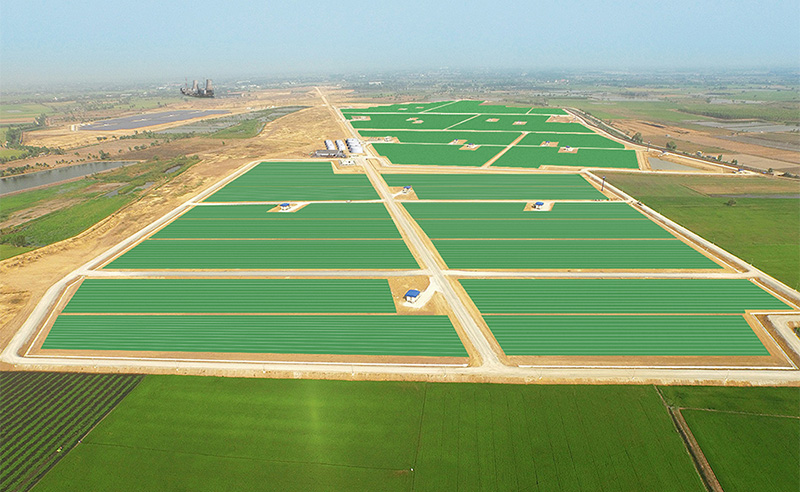
\includegraphics[width = 200px]{terrenos verdes.jpg}}
    \hfill
    \subfloat[Edifício. \label{fig: edificio}]{
        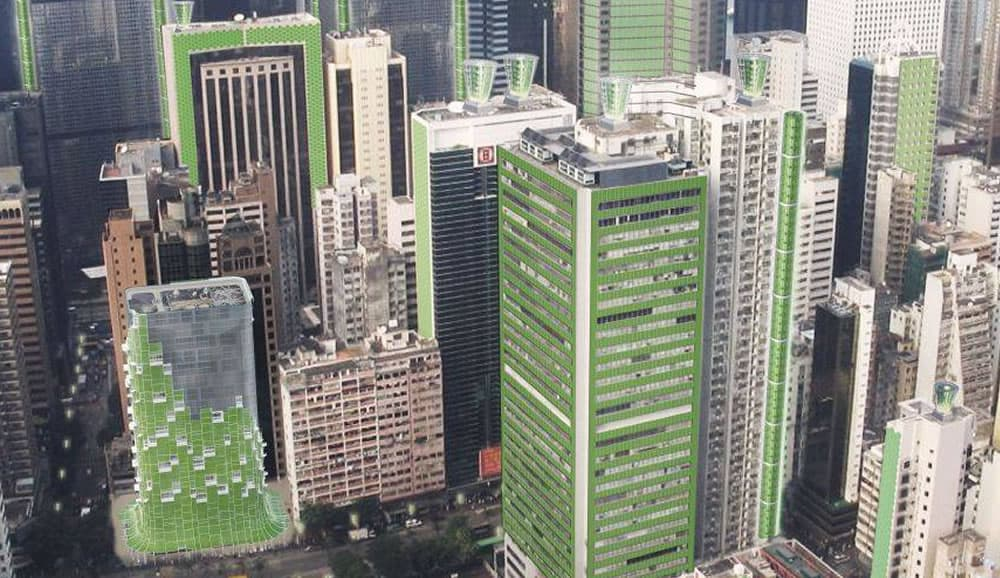
\includegraphics[width = 200px]{edificios verdes.jpg}}
\end{figure}
\par Desta forma pode-se matar não só 2 coelhos numa só cajadada, mas sim 3 (Reduzir CO2, Aumentar O2, Produz alimento), este projeto garante uma estimativa de produzir oxigénio respirável a uma taxa equivalente a 100 árvores em uma pequena superfície, porém, esse não é o principal objetivo, e sim criar mais proteína de forma ecológica, mais fontes de antioxidantes e corantes alimentares naturais.

%%%%%%%%%%%%%%%%%%%%%%%%%%%%%%%%%%%%%%%%%%%%%
%%%%%%%%%%%%%%%%%%%%%%%%%%%%%%%%%%%%%%%%%%%%%
\newpage
\underline{PRODUÇÃO DE ENERGIA}
\vspace{0.5cm}
\par \citep{cerri_sistema}Este é um novo método de {\bf energia renovável}, ou seja, a partir de algas que filtram água residual, tal como, a própria para tomar banho, lavar a loiça e roupa etc, tendem a crescer em *\hyperlink{thesentence}{fotobiorreatores}.
\par Quando essas algas estão prontas, são colhidas, transformadas em biomassa, através de um processo de incineração ("cremadas"), finalmente daí resulta a fonte energética que alimenta os sistemas do prédio, nesse processo não são utilizados químicos, logo a água é reaproveitada, e eventualmente pode ser usada como “greywater”, isto é, para uso doméstico e não consumível desse prédio.
\par Caso queira assistir a um vídeo mais detalhado acerca do assunto.
%%%%%%%%%%%%%%%%%%%%%%%Video%%%
\begin{center}
\fbox{\href{https://www.youtube.com/watch?v=butUX_VmJ54&feature=emb_logo&ab_channel=OriginClear}{Clique Aqui}}
\end{center}
%%%%%%%%%%%%%%%%%%%%%video%%%%
\par O projeto ajuda a eliminar as emissões, a economizar dinheiro e água que seria desperdiçada pelo ralo fora. Segundo os dados obtidos em França comprova-se que é muito eficiente não só pelo sua capacidade de gerar energia equivalente ao do carvão, mas também porque é considerado um método mais barato e limpo do que os outros meios para obter energia. Utiliza apenas {\bf luz}, {\bf gás carbónico} e {\bf águas residuais}.\\[0.3cm]
\begin{figure}[h!]
    \centering
    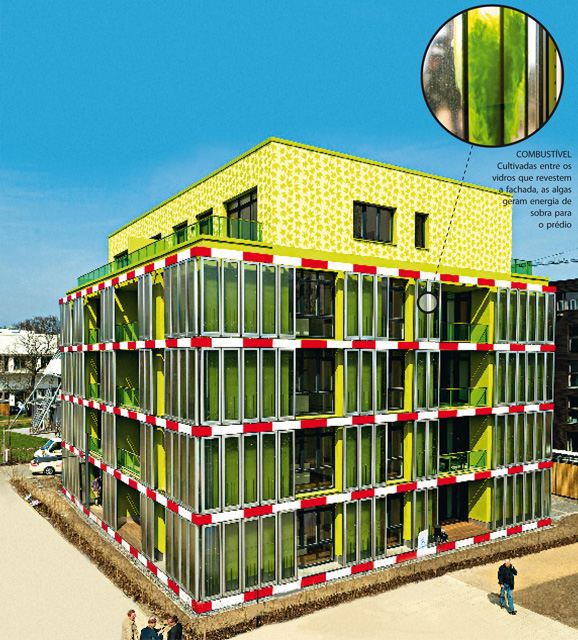
\includegraphics[width = 200px, height = 150px]{algas.jpg}
    \caption{Exemplo de uma obra com a aplicação deste projeto}
    \label{fig:algas}
\end{figure}
\par*\hypertarget{thesentence}{\textcolor{blue}{fotobiorreatores}}: Painéis instalados em ambientes fechados ou abertos, necessitando de luz artificial ou solar, caso os tubulares sejam ligados em série, podem diminuir os gases causadores de efeito estufa.
%%%%%%%%%%%%%%%%%%%%%%%%%%%%%%%
%%%%%%%%%%%%%%%%%%%%%%%%%%%%%%%
\newpage
\section{Pegada Ecológica}
\vspace{0.5cm}
\par \citep{ecycle_o, sardinhadossantos_pegada}Conhecida também por \textbf{pegada ambiental} é um método que determina o consumo da população e da sua respetiva localidade apresentando também um limite ecológico do nosso planeta, por outras palavras, ajuda a perceber se este suporta o estilo de vida da humanidade. Estatisticamente, observa-se que as \underline{áreas com maior industrialização} apresentam uma pegada considerável, ou seja, temos que tomar mais precauções nesses espaços.
\par Criado por William Rees e Mathis Wackernagel nos anos 90, onde aproveitaram para lançar um livro relacionado com a pertinência da sustentabilidade.
\par O cálculo da Pegada Ecológica total permite converter as áreas para {\bf hectares}, é realizado através da soma dos diferentes territórios produtores do planeta, estes são nomeados como {\bf subpegadas}, por exemplo:
\begin{description}
    \item[Retenção de carbono:] Espaço planeado para a reflorestação devido à dependência do oxigénio e diminuição do material originado pela madeira; 
    \item[Pastagem:] Região da criação de gado;
    \item[Florestal:] Espaço para produzir madeira e combustíveis
    \item[Pesqueiros:] Baseado na piscicultura, isto é, sustentar e criar peixes capturados dos meios aquáticos;
    \item[Áreas de cultivo:] Destinado ao cultivo de nutrientes e fibras (Humanos) e rações (Animais);
    \item[Áreas construídas:] Áreas onde provêm infraestruturas, reservadas para uma maior atividade e movimento, resumindo por outras palavras, são as cidades.
\end{description}
%%%%%%%%%%%%%%%%%%%%%%%%%%%%%%%%
%%%%%%%%%%%%%%%%%%%%%%%%%%%%%%%%
\newpage
\par Esta operação permite-nos ajudar o nosso planeta, pelo que, é um facto que não é possível adivinhar o futuro, no entanto, a pegada ajuda a obter uma ideia da sua condição presumível dentro de um estimado tempo, para o caso do modelo do cálculo permanecer inalterado. Portanto, a pegada alerta-nos, de forma a ganharmos \hypertarget{thesentence1}{\underline{atitude}} e gerir as nossas vidas em prol das nossas necessidades para que não excedam os limites dos ecossistemas.\\[0.3cm]
\par Na seguinte tabela \ref{tab:peg} será apresentada a relação entre a pegada ecológica e a biocapacidade da Terra ao longo dos anos, indicando a verde uma exigência humana igual ou inferior a um planeta e a vermelho superior, o que revela uma sobrecarga sobre ele.\\[0.5cm]
%%%%%%%%%%%%%%%%tabela%%%%%%%%%%%%%%%%
\begin{table}[h!]
    \centering
    \setlength{\arrayrulewidth}{1mm} 
    \setlength{\tabcolsep}{18pt} 
    \begin{tabular}{|c|c|c|c|c|}
        \hline 
        \multicolumn{5}{| c |}{Razão}  \\ 
        \hline 
        1961 & 1965 & 1970 & 1975 & 1980 \\ 
        \cellcolor[HTML]{66FF66} 0,74 & \cellcolor[HTML]{66FF66} 0,85 & \cellcolor[HTML]{66FF66} 1,00 & \cellcolor[HTML]{FF6666} 1,08 & \cellcolor[HTML]{FF6666} 1,16\\
        \hline 
        1985 & 1990 & 2000 & 2005 & 2008 \\
        \cellcolor[HTML]{FF6666} 1,14 & \cellcolor[HTML]{FF6666} 1,25 & \cellcolor[HTML]{FF6666} 1,30 & \cellcolor[HTML]{FF6666} 1,45 & \cellcolor[HTML]{FF6666} 1,52 \\
        \hline
    \end{tabular} 
    \caption{Dados aproximados da pegada ecológica nos respetivos anos}
    \label{tab:peg}
\end{table}
\vspace{0.5cm}
%%%%%%%%%%%%%%Tabela%%%%%%%%%
\par A iniciativa da mencionada \hyperlink{thesentence1}{atitude} consiste nas {\bf rotinas} de cada um de nós, ou seja, um bom primeiro passo a dar, é a nossa {\bf reavaliação diária}, de seguida, organizar de forma a ajustar e melhorar o nosso estilo. A partir, desse momento é uma questão de gerir o tempo e de poupar, não só economicamente, mas também no aspeto de usar apenas os recursos naturais necessários, por exemplo, reduzir o uso de água e energia, evitar o uso de transportes pessoais, optando maioritariamente pelos meios de transporte públicos, bicicleta (Exemplo de iniciativa: \href{http://uaubike.web.ua.pt/pt}{UauBike}) ou até mesmo a pé, reciclar material, entrar em listas de voluntariados, entre outras atividades que podem fazer a diferença.
\par Em modos de finalizar este capítulo sugere-se um site, que permite calcular através de um {\bf inquérito} a pegada ecológica individual, com intuito de nos fazer refletir e alterar os nossos comportamentos consumistas. Para isso clique
\href{https://www.wwf.org.br/natureza_brasileira/especiais/pegada_ecologica/sua_pegada/calculadora/}{aqui}! Depois de entrar no site volte a clicar sobre o texto \underline{"Você pode calcular sua Pegada Ecológica no site"}.

%%%%%%%%%%%%%%%%%%%%%%%%%%%%%%%%
%%%%%%%%%%%%%%%%%%%%%%%%%%%%%%%%
\newpage
\section{Estimativa dos Impactos}
Considerando tudo o que foi mencionado até agora, faz sentido mostrar a evolução esperada de alguns dos tópicos abordados.\\[0.1cm]
\par \citep{a2020_world}Começaremos por apresentar uma tabela \ref{Tabela 1:população} referente ao aumento da população ao longo dos anos. Mesmo parecendo inofensivo, se for a um ritmo acelerado, trás grandes consequências ao ambiente. Isto ocorre devido a serem precisos mais {\bf recursos para sustentar} toda a gente adicional que agora existe, logo cortam-se mais árvores, é necessária mais {\bf área habitacional} e {\bf comida}, entre muitas outras coisas.
%%%%%%%%%%%%%%%%tabela%%%%%%%%%%%%%%%%
\begin{table}[h!]
\centering
 \begin{tabular}{||c | c c c c||} 
 \hline
 Ano & 1990 & 2000 & 2010 & 2020 \\ [0.5ex] 
 \hline
 Bilião & 5,3 & 6,1 & 6,9 & 7.8 \\ [1.0ex]
 \hline
 \end{tabular}
 \caption{Aumento da População}
 \label{Tabela 1:população}
 \end{table}
%%%%%%%%%%%%%%%%tabela%%%%%%%%%%%%%%%%
\par Como é possível evidenciar na tabela \ref{Tabela 1:população}, num espaço de tempo inferior a 40 anos, {\bf a população  aumentou um total 3 biliões de pessoas}.\\[0.5cm]
\par \citep{vasconcelos_2019_planeta}A próxima tabela diz respeito à quantidade de plástico criado anualmente e uma previsão de quanto plástico estaremos a criar em 2030.
%%%%%%%%%%%%%%%%tabela%%%%%%%%%%%%%%%%
 \begin{table}[H]
\centering
 \begin{tabular}{||c | c c c c||} 
 \hline
 Ano & 1980 & 2000 & 2016 & 2030 \\ [0.5ex] 
 \hline
 Milhões de Toneladas & 70 & 213 & 396 & 550 \\ [1.0ex]
 \hline
 \end{tabular}
 \caption{Criação de Plástico}
 \label{Tabela 2:produção plástico}
 \end{table}
%%%%%%%%%%%%%%%%tabela%%%%%%%%%%%%%%%%
\par \citep{natgeoportugal_2020_sem}
Escusado será dizer que, dado aos facto do plástico não ser biodegradável e ser dificilmente reutilizável (devido à existência de micro plásticos nocivos aos seres humanos), estes causam uma grande parte da poluição no planeta, sendo o {\bf maior poluente dos oceanos}, neste preciso momento. 
\newpage
%%%%%%%%%%%%%%%%tabela%%%%%%%%%%%%%%%%
\begin{table}[H]
\begin{center}
 \begin{tabular}{||c | c c ||} 
 \hline
 Ano & 2015 & 2040 \\ [0.5ex] 
 \hline
 Milhões & 150 & 600 \\ [1.0ex]
 \hline
 \end{tabular}
 \caption{Quantidade de Plástico nos Oceanos}
 \label{Tabela 3:plástico oceanos}
 \end{center}
 \end{table}
 %%%%%%%%%%%%%%%%tabela%%%%%%%%%%%%%%%%
A tabela que acabamos de visualizar tem uma estimativa da quantidade de plástico à deriva nos oceanos, tanto no ano de 2015, como a que se prevê para o caso de continuarmos sem qualquer tipo de precaução com a {\bf produção} e o {\bf descartamento} deste.
\par Como era expectável, estes valores são catastróficos de um ponto de vista ambiental, e, caso a suposição se realize, agrava extremamente a situação já trágica das mudanças climatéricas presentes na atualidade.
%%%%%%%%%%%%%%%%%%%%%%%%%%%%%%%%%%%%%%%%
\section{Conclusão e Recomendação}
Com base em toda a informação que adquirimos através da realização deste trabalho, apesar de ainda ser bastante superficial, tendo em conta a enorme {\bf abrangência} e {\bf complexidade} deste tema. Poderia abordar \underline{literalmente tudo} o que nos rodeia, porque quase todo o material no dias atuais sofre, efetivamente, um processo prejudicial ao ambiente, por exemplo, uma simples peça de roupa, desde a sua produção até ser descartada pelo seu utilizador contribui significativamente para impactos ambientais negativos, sentidos sobretudo ao nível da {\bf desflorestação e erosão dos solos} (cultivo da planta do algodão), da {\bf emissão de CO2} (Transportes e produção de roupa nas fabricas), {\bf consumo da água em excesso} (Lavagens de roupa), dos {\bf resíduos} (durante a lavagem são lançados para o mar produtos tóxicos resultantes do detergente, das roupas e ainda microplásticos) e desperdícios resultantes.
Em suma, trazemos aqui não só aspetos negativos, mas também referências a seguir, que servem de partido a muitas outras ideias inovadoras. Diz-se que {\bf \underline{o cérebro é uma máquina que faz magia}}, por isso recomenda-se que, com seriedade, encaremos o grave estado do nosso planeta e assuma-se uma postura mais correta para reverter todo o impacto negativo causado.
%%%%%%%%%%%%%%%%%%%%%%%%%%%%%%%%%%%%%
\newpage
\Large{\bf Contribuições}
\begin{itemize}
    \item Rafael Amorim: 65\%
    \begin{enumerate}
        \item Inovações Tecnológicas
        \item Relógio do Clima
        \item Enzima que consome plástico
        \item Comboios de Energia Eólica
        \item Painel Verde
        \item Pegada Ecológica
        \item Conclusão e Recomendações
        \item Bibliografia
    \end{enumerate}
    \item Gonçalo Sousa: 35\%
    \begin{enumerate}
        \item Introdução
        \item Meio Ambiente
        \item Sistema de Ocean Clean Up
        \item Roupas Energéticas
        \item Estimativa dos Impactos
    \end{enumerate}
\end{itemize}
%%%%%%%%%%%%%%%%%Bibliografia%%%%%%%%

\bibliographystyle{plain}
\bibliography{myBib}

\end{document}